\documentclass[10pt,final,conference]{IEEEtran}
%\IEEEoverridecommandlockouts
% The preceding line is only needed to identify funding in the first footnote. If that is unneeded, please comment it out.
\usepackage{amsmath,amssymb,amsfonts,amsthm}
\usepackage{graphicx}
\usepackage{textcomp}
\usepackage{xcolor}
\usepackage{siunitx}
\usepackage{mathtools}
\usepackage{booktabs,array}
\usepackage{algorithm,setspace}
\usepackage{algorithmic}
\usepackage[T2A]{fontenc}
\usepackage[utf8]{inputenc}
\usepackage[numbers,sort&compress]{natbib}
\def\BibTeX{{\rm B\kern-.05em{\sc i\kern-.025em b}\kern-.08em
    T\kern-.1667em\lower.7ex\hbox{E}\kern-.125emX}}

\renewcommand{\sfdefault}{cmss}
\renewcommand{\rmdefault}{cmr}
\renewcommand{\ttdefault}{cmt}

\makeatletter
\renewcommand*\env@matrix[1][\arraystretch]{%
	\edef\arraystretch{#1}%
	\hskip -\arraycolsep
	\let\@ifnextchar\new@ifnextchar
	\array{*\c@MaxMatrixCols c}}
\makeatother

\DeclareRobustCommand{\rchi}{{\mathpalette\irchi\relax}}
\newcommand{\irchi}[2]{\raisebox{\depth}{$#1\chi$}}

\newtheorem{lemma}{\textbf{Lemma}}
\newtheorem{assumption}{\textbf{Assumption}}
\renewenvironment{proof}{{\noindent\it Proof.}\quad}{\hfill $\square$\par}

\renewcommand{\algorithmicrequire}{\textbf{Input:}} 
%Use Input in the format of Algorithm
\renewcommand{\algorithmicensure}{\textbf{Output:}} %UseOutput in the format of Algorithm

\allowdisplaybreaks[4]


\begin{document}

\title{Trajectory and Power Control for UAVs \\ Project Report\\
%{\footnotesize \textsuperscript{*}Note: Sub-titles are not captured in Xplore and
%should not be used}
%\thanks{Identify applicable funding agency here. If none, delete this.}
}

\author{\IEEEauthorblockN{1\textsuperscript{st} Xiaopeng Li}
\IEEEauthorblockA{\textit{Math Department} \\
\textit{CUHK(SZ)}\\
Shenzhen, China \\
116010114@link.cuhk.edu.cn}
\and
\IEEEauthorblockN{2\textsuperscript{nd} Yihan Huang}
\IEEEauthorblockA{\textit{Electronic Info Engineering Department} \\
\textit{CUHK(SZ)}\\
Shenzhen, China \\
117010101@link.cuhk.edu.cn}
\and
\IEEEauthorblockN{3\textsuperscript{rd} Chenhao Wu}
\IEEEauthorblockA{\textit{Computer Science Department} \\
\textit{CUHK(SZ)}\\
Shenzhen, China \\
117010285@link.cuhk.edu.cn}
}

\maketitle

\begin{abstract}
	In this paper, we consider $K$ unmanned aerial vehicles (UAVs) communicating with their corresponding base stations (BSs) at the same time and over the same spectrum. To reduce the interference and achieve the maximum channel capacity over all UAVs, we formulate a trajectory power control problem (TPC) for certain time horizon with height, velocity and collision avoidance constriants, which leads to a large-scale non-convex optimization problem. By scrutinizing the structure of the TPC problem, we verify that the optimal solution should follow the fly-hover-fly strategy. This strategy can be solved heuristically by first finding the hovering location, and then solving dimension-reduced TPC problem with the given hovering location. For the TPC problem, we purpose a successive convex approximation algortihm to solve it. Simulation results indicated our method achieve higher channel capacity and higher compuation time efficiency than the benchmark strategy.
\end{abstract}
\vskip 1ex

\begin{IEEEkeywords}
	UAV, trajectory design, power control, collision avoidance, interference channel, successive convex approximation
\end{IEEEkeywords}

\section{Introduction}\label{I}
An unmanned aerial vehicle (UAV) is an aerial vehicle that can fly autonomously or controlled by a ground station to execute military, commerical or civilian tasks \cite{IEEEexample:shen2018multi,IEEEexample:zeng2016wireless}. Due to its higher agility, better communication channels, and flexible reconfiguration, UAVs are widely used in ubiquitous coverage, relaying, and information dissenmination and data collection \cite{IEEEexample:zeng2016wireless}. However, unlike the conventional wireless communication systems with static base stations (BSs), which only need power control for attaining required signal quality, UAV-enabled wireless communications often require joint trajectory planning and communication power control. This is mainly because the UAV is energy-constrained. Besides, collision avoidance and interference management are also essential for multi-UAV scenario.

There have been a growing body of research on UAV-enabled wireless communication systems. Reference \cite{IEEEexample:7888557} considered optimization on energy and trajectory for single UAV-BS pair. Reference \cite{IEEEexample:li2019uav} solved joint positioning and power control for multi-UAV system. In this paper, we study a interference channel, where $K$ UAVs communicate with their respective BSs simultanenously over the same spectrum. To maximize the channel capacity when dynamic interference control is allowed, we formulate such scenario as a UAV trajectory and power control (TPC) problem, which also takes collision avoidance into consideration.

The TPC problem we formulated has two main challenges. Firstly, the problem is NP-hard because the objective function and collision avoidance constraint are nonconvex. Secondly, due to the avoidance constraint, the number of time slots should be large enough, and combined with the large number of UAVs, the problem dimension could be very large. In this paper, we discover two properties of TPC problem to reduce the problem dimension and derive a tight surrogate concave function to invoke the successive convex approximation method to solve the TPC problem efficiently.

The rest of the paper is organized as follows. Section \ref{II} presents the model formulation of TPC optimization problem for maximizing channel capacity. The strategy for solving the TPC problem is analyzed in Section \ref{III}. In Section \ref{IV}, a customized SCA algorithm is presented for solving TPC problem efficiently. The simulation results are displayed in Section \ref{V} and the work is concluded in Section \ref{VI}.
\vskip 1\baselineskip

\section{Problem Formulation}\label{II}
Consider $K$ UAVs communicating with their associated base stations (BSs) at the same time over the same spectrum. First, we only consider the downlink communication from the UAVs to BSs. Assume that both UAVs and BSs only have one antenna that can receive and transmit signal in all directions. Denote the fixed BS position matrix as $\boldsymbol{s}\in\mathbb{R}^{3\times K}$, and for the $k$-th UAV, the position of it is $\boldsymbol{s}_{[:,k]}\in\mathbb{R}^3,\,\forall\,k\in\mathcal{K}$, where $\mathcal{K}\triangleq\{1,\ldots,K\}$. We discretized the whole time horizon $T$ into $N$ time slots with equal length, i.e., $T=NT_s$, and $T_s$ is the length of each time slots. Denote $\boldsymbol{q}\in\mathbb{R}^{3\times K\times (N+2)}$ as the location tensor for UAVs, and $\boldsymbol{q}_{[:,k,n+1]}\in\mathbb{R}^3$ for $n\in\mathcal{N}_1^N$ as the location of $k$-th UAV at time slot $n$, where $\mathcal{N}_i^j=\{i,\ldots,j\}$ for $1\leq i\leq j\leq N+2$. Notice that here, $\boldsymbol{q}_{[:,k,1]}$ and $\boldsymbol{q}[:,k,N+2]$ are the initial and final location (which are given values, not decision variables) of the $k$-th UAV, respectively. 

Denote $H_{\min}$ and $H_{\max}$ as the minimum and maximum safe altitude for all UAVs, then we have the following flying altitude constraints,
\begin{equation}\label{Eq1}
H_{\min}\leq\boldsymbol{q}_{[3,k,n+1]}\leq H_{\max}
\end{equation}
where $\boldsymbol{q}_{[3,k,n+1]}\in\mathbb{R}$ is the third entry of vector $\boldsymbol{q}_{[:,k,n+1]}$.

Due the the limited flight speed of UAVs, we need to put several constraints on the distance between different positions of one UAV in any two consecutive time slots. Denote the level-flight speed, vertical ascending and descending speed (m/s) as $V_L,V_A,V_D$ repsectively, then the position constraints for a single UAV is
\begin{subequations}
	\begin{equation}\label{Eq2.1}
	\left\lVert\boldsymbol{q}_{[1:2,k,n+1]}-\boldsymbol{q}_{[1:2,k,n]}\right\rVert\leq V_LT_s
	\end{equation}
	\begin{equation}\label{Eq2.2}
	-V_DT_s\leq\boldsymbol{q}_{[3,k,n+1]}-\boldsymbol{q}_{[3,k,n]}\leq V_AT_s
	\end{equation}
\end{subequations}
where $\boldsymbol{q}_{[1:2,k,n+1]}\in\mathbb{R}^2$ denotes the subvector of $\boldsymbol{q}_{[:,k,n+1]}$ by taking only the first two entries.

Also, we need to consider the collision avoidance of any two UAVs. If the minimum safe distance between any two UAVs is denoted by $d_{\min}$, we have the collision avoidance constraints
\begin{equation}\label{Eq3}
\left\lVert\boldsymbol{q}_{[:,k,n+1]}-\boldsymbol{q}_{[:,j,n+1]}\right\rVert\geq d_{\min}
\end{equation}
Finally, the transmission power of all the UAVs must be bounded. Denote $\boldsymbol{p}\in\mathbb{R}^{k\times (N+2)}$ as the power matrix, and $\boldsymbol{p}_{[k,n+1]}\in\mathbb{R}$ as the transmission power of $k$-th UAV at time slot $n$, $\forall\,k\in\mathcal{K},n\in\mathcal{N}_1^N$, then we have the power constraints
\begin{equation}\label{Eq4}
0\leq \boldsymbol{p}_{[k,n+1]}\leq P_{\max}
\end{equation}
where $P_{\max}$ denotes the maximum transmission power of all UAVs. We also denote $\boldsymbol{p}_{[k,1]}$ and $\boldsymbol{p}_{[k,N+2]}$ as the initial and final transmission power (which are given values, not decision variables).

After deriving the constraints for our trajectory and power control (TPC) problem, we now consider the objective function we need to maximize. However, to be more rigorous, we list out the main assumptions for UAV-based wireless communication in this paper.
\begin{assumption}\label{assumpt1}
	We assume the following assumptions hold throughout this paper,
	\begin{enumerate}
		\item The UAVs are communicating with BSs in rural area at moderate altitude. Furthermore, the radio wave is only considered to traverse through Line-of-sight link and will not be blocked by any obstacles. 
		\item The Doppler effect can be ignored. This assumption is reasonable when the speed of UAVs are not large.
	\end{enumerate}
\end{assumption}
Now we are ready to derive the objective function. If we denote the channel capacity (bits/second) matrix as $R\in\mathbb{R}^{K\times (N+2)}$, then the channel capacity of $k$-th UAV at time slot $n$ is $R_{[k,n+1]}\in\mathbb{R}$, for $k\in\mathcal{K}$ and $n\in\mathcal{N}_1^N$. Thus, the objective function can be written as
\begin{equation}\label{Eq5}
\max_{\substack{\boldsymbol{p}_{[:,2:N+1]},\\ \boldsymbol{q}_{[:,:,2:N+1]}}}\quad\sum_{n=2}^{N+1}\sum_{k=1}^K R[k,n]
\end{equation}
Notice that the channel capacity can be calculated by Shannon-Hartley Theorem, i.e.,
\begin{equation}\label{Eq5.1}
R_{[k,n]} = B\log_2\left(1+\text{SNR}_{[k,n]}\right)\tag{5.1}
\end{equation}
where $B$ (Hertz) is the bandwidth of the channel. Under Assumption \ref{assumpt1}, it is reasonable to adopt the Free-space path loss (FSPL) radio energy attenuation model, and thus the channel gain between $j$-th UAV and $k$-th BS at time slot $n$ is given by
\begin{equation}\label{Eq5.2}
G_{[j,k,n+1]}=\frac{G_0}{\lVert\boldsymbol{q}_{[:,j,n+1]}-\boldsymbol{s}_{[:,k]}\rVert^2}\tag{5.2}
\end{equation}
where $G_0$ (watt) is the channel gain between any UAV and BS at the distance of one meter; $G\in\mathbb{R}^{K\times K\times (N+2)}$ is the channel gain tensor. Thus, by definition of SNR (signal-to-noise ratio), we have 
\begin{equation}\label{Eq5.3}
\text{SNR}_{[k,n]} = \frac{G_{[k,k,n]}\boldsymbol{p}_{[k,n]}}{BN_0+\sum_{j=1,j\ne k}^{K}G_{[j,k,n]}\boldsymbol{p}_{[j,n]}}\tag{5.3}
\end{equation}
where $N_0$ is the power spectral density (PSD) of the additive white Gaussian noise (AWGN).

Therefore, combine (\ref{Eq1})-(\ref{Eq5}), we can write down the formulation of TPC optimizaiton problem as
\begin{equation}\label{Eq6}
\begin{array}{cll}
	\max\limits_{\substack{\boldsymbol{p}_{[:,2:N+1]},\\ \boldsymbol{q}_{[:,:,2:N+1]}}}\quad & \sum\limits_{n=2}^{N+1}\sum\limits_{k=1}^K R_{[k,n]}(\boldsymbol{p},\boldsymbol{q}) \\ 
	s.t. \quad & (\ref{Eq1}),(\ref{Eq4})\ \forall\,k\in\mathcal{K},n\in\mathcal{N}_1^N \\
	& (\ref{Eq2.1}),(\ref{Eq2.2}),\ \forall\,k\in\mathcal{K},n\in\mathcal{N}_1^{N+1} \\
	& (\ref{Eq3}),\ \forall\,k,j\in\mathcal{K},k<j,n\in\mathcal{N}_1^N
\end{array}
\end{equation}

At the very end of this chapter, we tend to declare two addtional requirements for the parameter settings in (\ref{Eq6}). One thing is that we assume each UAV should return to its initial position, i.e.,
\begin{equation}\label{6.1}
\boldsymbol{q}_{[:,k,1]} = \boldsymbol{q}_{[:,k,N+2]},\ \forall\,k\in\mathcal{K}\tag{6.1}
\end{equation}
The other thing is that the length of each time slots cannot be to long, i.e., $T_s$ should be bounded above by some value. This is because we assume the UAVs keep their position and transmission power unchanged within a single time slot, but in reality if $T_s$ is too long, two UAVs may collide with each other within the single time slot. This implies that $T_s$ should be short enough so that in extreme case (two UAVs flying towards each other with maximum net speed), any two UAVs will not collide, with the shortest possible initial distance (minimum safe distance).
\begin{equation}\label{6.2}
T_s \leq \frac{d_{\min}}{\sqrt{4V_L^2+(V_A+V_D)^2}}\tag{6.2}
\end{equation}
\vskip 1\baselineskip

\section{Reformulation and Strategy}\label{III}
The difficulty of problem (\ref{Eq6}) lies in two sides. For one thing, it is not hard to see that problem (\ref{Eq6}) is a non-convex optimization problem, which is too hard to solve directly. This indicates that we need to do some relaxation to reformulate it into a tractable and solvable problem, which admits low time complexity to solve. For the other thing, from (\ref{6.2}) we can see that when the number of time slots are large, the dimension of this optimization problem would be too large. Thus, we also need some dimension-reducing method and find some special property of the optimization problem (\ref{Eq6}) to shrink the problem dimension. With out loss of generality (W.O.L.G.), in the remaining part of our paper, we will assume the number of timeslots $N$ is odd.

Firstly, we derive some properties that can help reduce the dimension of (\ref{Eq6}). From our assumption in (\ref{6.1}), it is intuitive to think that the optimal flying trajectory should be symmetric. Fortunately, our intuition here is true as long as the ascending and descending speed are equal. The verification is given in the following lemma.
\begin{lemma}\label{lemma1}
	Assume {\rm (\ref{6.1})} holds, and the ascending and descending speed are equal, i.e., $V_A=V_D$. Denote one of the optimal solution of problem {\rm (\ref{Eq6})} as $\boldsymbol{q}^*$ and $\boldsymbol{p}^*$, then for all $k\in\mathcal{K}$, we have
	\begin{equation}\label{Eq7}
	\boldsymbol{q}^*_{[:,k,n]} = \boldsymbol{q}^*_{[:,k,N+3-n]},\ \boldsymbol{p}^*_{[k,n]} = \boldsymbol{p}^*_{[k,N+3-n]},\ \forall\,n\in\mathcal{N}_2^{N+2}
	\end{equation}
\end{lemma}
\begin{proof}
	We first define ${R_s}_{[n]} \triangleq \sum_{k=1}^K R_{[k,n]}(\boldsymbol{p}^*,\boldsymbol{q}^*)$, and let
	$R_1 = \sum_{n=2}^{(N+1)/2}{R_s}_{[n]}$ and $R_2 = \sum_{n=(N+1)/2+1}^{N+1}{R_s}_{[n]}$.
	W.O.L.G., assume $R_1>R_2$, then assigning the trajectory and transmission power solutions of each UAV at time slot $n$ to time slot $N+3-n$ for any $n=2,\ldots,(N+1)/2$ will yield total objective function value of $2R_1>R_1+R_2$. Also, since $V_A=V_D$, all constraints in (\ref{Eq6}) will be satisfied for this newly assigned trajectory and power solutions. This is because as long as $V_A=V_D$, all constraints are symmetric for any two consecutive time slots. Therefore, any optimal solution must satisfy $R_1=R_2$, and at least one of optimal solution is symmetric, i.e., will satisfy (\ref{Eq7}).
\end{proof}
\vskip 1\baselineskip
In pratice, we notice that the UAVs are not always flying, instead it usually flies to some location and hovers there, until afterwhile it has to return due to the requirement that it needs to fly back to the orginal location at the end of time horizon $T$. To explore this phenomenon, we have the following lemma.
\begin{lemma}\label{lemma2}
	Using the same notations in {\rm Lemma \ref{lemma1}}, for some $M_0\in\{2,3,\ldots,N+1\}$ and $M\in\{2,3,\ldots,M_0\}$, we have
	\begin{equation}\label{Eq8}
	{R_s}_{[n]}\leq {R_s}_{[M]}={R_s}_{[M+1]}=\cdots={R_s}_{[M_0]},\ \forall\,n\in\mathcal{N}_2^M
	\end{equation}
	where $M_0$ is the time when the UAVs need to return from the hovering location, and $M$ is the time when UAVs arrives the hovering location. In particular, if $V_A=V_D$, $M_0=N+3-M$.
\end{lemma}
\begin{proof}
	Suppose (\ref{Eq8}) does not hold and the optimal objective value for the first $M_0$ slots (the existence of $M_0$ is trivial because the $k$-th UAV must return to the original location $\boldsymbol{q}_{[:,k,N+2]}$) is $\sum_{n=2}^{M_0} {R_s}_{[n]}$.
	Due to the constraints (\ref{Eq1}), (\ref{Eq2.1}), (\ref{Eq2.2}), and (\ref{Eq4}), we can conclude that ${R_s}_{[n]}$ is bounded for all $n\in\mathcal{N}_2^{N+1}$. Thus, there exists some $M\in\{2,3,\ldots,M_0\}$ such that ${R_s}_{[M]}=\max\{{R_s}_{[2]},\ldots,{R_s}_{[M_0]}\}$. Thus, we have
	$(M_0-M+1){R_s}_{[M]}\geq \sum_{n=M}^{M_0} {R_s}_{[n]}$, 
	which implies that by keeping the trajectory and power of UAV at time slot $M$ for the following $M_0-M$ slots we can achieve an objective value that is no worse than the objective value when (\ref{Eq8}) does not hold. Also, this strategy will not violate any constaints in (\ref{Eq6}), because the trajectory and power of each UAV at time slot $M$ is a feasible solution of (\ref{Eq6}). This is a contradiction which shows that (\ref{Eq8}) must hold.
	If $V_A=V_D$, we can apply Lemma \ref{lemma1}, and the trajectory and power solution for the time horizon $T$ will be symmetric. Thus, by (\ref{Eq7}), we can easily shows that $M\in\{2,3,\ldots,(N+1)/2\}$ and $M_0+M=N+3$.
\end{proof}

Thus, in general, Lemma \ref{lemma2} tells us that the optimal strategy for all UAVs should be that the UAVs first fly to location $\boldsymbol{q}_{[:,k,M]}$, where it attains the maximum objective value ${R_s}_{[M]}$ along the trajectories, and hover until time slots $M_0$, and then fly back. For simplicity, now we only consider the case when $V_A=V_D$. In this case, problem (\ref{Eq6}) can be reduced to
\begin{equation}\label{Eq9}
	\begin{array}{cll}
		\max\limits_{\substack{\boldsymbol{p}_{[:,2:M]}, \\ \boldsymbol{q}_{[:,:,2:M]}, \\ M\in\mathcal{N}_2^{(N+1)/2}}}\quad & \sum\limits_{n=2}^{M}\sum\limits_{k=1}^K R_{[k,n]}(\boldsymbol{p},\boldsymbol{q}) \\[-20pt] &\qquad+\left(\frac{N+1}{2}-M\right)\sum\limits_{k=1}^KR_{[k,M]}(\boldsymbol{p},\boldsymbol{q}) \\
		s.t. \quad & (\ref{Eq1}),(\ref{Eq2.1}),(\ref{Eq2.2}),(\ref{Eq4}),\ \forall\,k\in\mathcal{K},n\in\mathcal{N}_2^M \\
		& (\ref{Eq3}),\ \forall\,k,j\in\mathcal{K},k<j,n\in\mathcal{N}_2^M
	\end{array}
\end{equation}
Notice that (\ref{Eq9}) is involved with solving an optimal $M$, which in general is difficult. Here, inspired by our observation, we use a heuristic method to solve the optimal $M$ and hovering location $\boldsymbol{q}_{[:,k,M]}$ for (\ref{Eq9}) first, and then use that fixed $M$ and $\boldsymbol{q}_{[:,k,M]}$ to solve (\ref{Eq9}). Since in the objective function in (\ref{Eq9}), the first term is much smaller than the second term when $N$ is much larger than $M$ (which is often true in practice), we can solve the approximation of optimal $M$ and $\boldsymbol{q}_{[:,k,M]}$ by omit the first term in objective function for problem (\ref{Eq9}), which is then simplified into
\begin{equation}\label{Eq10}
	\begin{array}{cl}
		\max\limits_{\substack{\boldsymbol{p}_{[:,M]}, \\ \boldsymbol{q}_{[:,:,M]}}} & \sum\limits_{k=1}^KR_{[k,M]}(\boldsymbol{p},\boldsymbol{q}) \\ 
		s.t. \quad & H_{\min}\leq\boldsymbol{q}_{[3,k,M]}\leq H_{\max}, \ \forall\,k\in\mathcal{K} \\
		& \left\lVert\boldsymbol{q}_{[1:2,k,M]}-\boldsymbol{q}_{[1:2,k,1]}\right\rVert\leq V_LT/2,\ \forall\,k\in\mathcal{K} \\
		& -V_DT/2\leq\boldsymbol{q}_{[3,k,M]}-\boldsymbol{q}_{[3,k,1]}\leq V_AT/2,\ \forall\,k\in\mathcal{K} \\
		&	\left\lVert\boldsymbol{q}_{[:,k,M]}-\boldsymbol{q}_{[:,j,M]}\right\rVert\geq d_{\min},\ \forall\,k<j,k,j\in\mathcal{K} \\
		& 0\leq \boldsymbol{p}_{[k,M]}\leq P_{\max},\  \forall\,k\in\mathcal{K}
	\end{array}
\end{equation}
Notice that in (\ref{Eq10}), we can only solve the approximated optimal hovering location with the corresponding transmission power there. Denote them as $\boldsymbol{q_h}^*_{[:,k]}\in\mathbb{R}^3$ and $\boldsymbol{p_h}^*_{[k]}\in\mathbb{R}$ for all $k\in\mathcal{K}$. Also denote $R_s^*=\sum_{k=1}^KR_{[k,M]}(\boldsymbol{p_h}^*_{[k]},\boldsymbol{q_h}^*_{[:,k]})$. Problem (\ref{Eq9}) reduces to
\begin{equation}\label{Eq11}
	\begin{array}{cl}
		\max\limits_{\substack{\boldsymbol{p}_{[:,2:M]}, \\ \boldsymbol{q}_{[:,:,2:M]} \\ M\in\mathcal{N}_2^{(N+1)/2}
		}} & \sum\limits_{n=2}^{M}\sum\limits_{k=1}^K R_{[k,n]}(\boldsymbol{p},\boldsymbol{q}) \\[-13pt] &\qquad+(\frac{N+1}{2}-M)R_s^* \\[5pt]
		s.t.  & (\ref{Eq1}),(\ref{Eq2.1}),(\ref{Eq2.2}),(\ref{Eq4}),\ \forall\,k\in\mathcal{K},n\in\mathcal{N}_2^M \\
		& (\ref{Eq3}),\ \forall\,k,j\in\mathcal{K},k<j,n\in\mathcal{N}_2^M \\
		& \boldsymbol{q}_{[:,k,M]}=\boldsymbol{q_h}^*_{[:,k]},\   \boldsymbol{p}_{[k,M]} = \boldsymbol{p_h}^*_{[k]},\  \forall\,k\in\mathcal{K}
	\end{array}
\end{equation}
Since all UAVs attains the maximum sum rate of channel capacity at their hovering location, if we assume $N\gg M$, the second term in objective function will be totally dominant. This implies that we need to find the smallest $M$ such that all UAVs can fly to the preset hovering locations without collision.
\begin{equation}\label{Eq12}
	\begin{array}{cll}
		\min\limits_{\substack{\boldsymbol{q}_{[:,:,2:M]}, \\ M\in\mathcal{N}_2^{(N+1)/2}}}\quad & M \\ 
		s.t. \quad & (\ref{Eq1}),(\ref{Eq2.1}),(\ref{Eq2.2}),\ \forall\,k\in\mathcal{K},n\in\mathcal{N}_2^M \\
		& (\ref{Eq3}),\ \forall\,k,j\in\mathcal{K},k<j,n\in\mathcal{N}_2^M \\
		& \boldsymbol{q}_{[:,k,M]}=\boldsymbol{q_h}^*_{[:,k]},\  \forall\,k\in\mathcal{K}
	\end{array}
\end{equation}
Notice that (\ref{Eq12}) is a nonconvex QCQP problem for each fixed $M$, which is hard to solve. To solve this efficiently, we can first remove the collision avoidance constraints, and (\ref{Eq12}) reduced to a convex QCQP problem, which is easy to solve. By using bisection method on $M$, we can find the smallest $M$ that 
makes this relaxed problem feasibile, denote it as $M_L$. Use $M_L$ as a lower bound for $M$, and apply bisection method over $M$ again, but on problem (\ref{Eq12}), we can find the optimal $M$ for (\ref{Eq12}). For method to check the feasibilty of (\ref{Eq12}), see Section \ref{IV} in details.
\vskip 1\baselineskip

\section{Algorithm}\label{IV}
Now we introduce the well-known successive convex approximation algorithm to deal with all nonconvex objective functions and constraints in the above section. For simplicity, we first declare some notations. Suppose at iteration $r$, the position and transmission power of the $k$-th UAV are denoted by $\boldsymbol{q}^r_{[:,k,n]}$ and $\boldsymbol{p}^r_{[k,n]}$ respectively. For all $k\in\mathcal{K}$ and $n\in\mathcal{N}_2^M$, define
\begin{subequations}
	\begin{equation}\label{Eq13a}
	\boldsymbol{a}^r_{[k,n]} \triangleq \sqrt{\boldsymbol{p}^r_{[k,n]}}, \ \boldsymbol{d}^r_{[j,k,n]} \triangleq \lVert\boldsymbol{q}^r_{[:,j,n]}-\boldsymbol{s}_{[:,k]}\rVert^2 
	\end{equation}
	\begin{equation}\label{Eq13b}
	\boldsymbol{a}_{[k,n]} \triangleq \sqrt{\boldsymbol{p}_{[k,n]}},\  \boldsymbol{d}_{[j,k,n]} \triangleq \lVert\boldsymbol{q}_{[:,j,n]}-\boldsymbol{s}_{[:,k]}\rVert^2 
	\end{equation}
	\begin{equation}\label{Eq13c}
	\boldsymbol{I}_{[k,n]} \triangleq \sum_{j=1, j\ne k}^K\frac{G_0(\boldsymbol{a}_{[k,n]})^2}{BN_0\boldsymbol{d}_{[j,k,n]}}
	\end{equation}
	\begin{equation}\label{Eq13d}
	\boldsymbol{I}^r_{[k,n]} \triangleq \sum_{j=1, j\ne k}^K\frac{G_0(\boldsymbol{a}^r_{[k,n]})^2}{BN_0\boldsymbol{d}^r_{[j,k,n]}}
	\end{equation}
\end{subequations}
Therefore, the channel capacity function can be defined as
\begin{equation}\label{Eq14}
	\begin{array}{rl}
		\overline{R}[k,n](\boldsymbol{a},\boldsymbol{q}) \triangleq & \log\left(1+\sum_{j=1}^K\frac{G_0(\boldsymbol{a}[k,j])^2}{BN_0\boldsymbol{d}[j,k,n]}\right)\\
		&\qquad-\log\left(1+\sum_{j=1,j\ne k}^K\frac{G_0(\boldsymbol{a}[k,j])^2}{BN_0\boldsymbol{d}[j,k,n]}\right)
	\end{array}
\end{equation}
Notice that $\frac{x^2}{y}$ is convex when $y>0$, $-\log(1+x)$ is convex when $x>-1$, and $x^2$ is convex for all $x\in\mathbb{R}$, thus we can find the global linear lower bound for them, i.e., for any fixed $\bar{x}$ in the function domain,
\begin{subequations}
	\begin{flalign}
		&\frac{x^2}{y} \geq \frac{2\bar{x}}{\bar{y}}x-\frac{\bar{x}^2}{\bar{y}^2}y,\ \text{for fixed }\bar{y}>0\label{15a} \\
		&-\log(1+x) \geq -\log(1+\bar{x}) - \frac{x-\bar{x}}{1+\bar{x}}\label{15b} \\
		&x^2 \geq 2x\bar{x}-\bar{x}^2\label{15c}
	\end{flalign}
\end{subequations}
Therefore, we can define the locally tight concave surrogate function of $\overline{R}_{[k,n]}(\boldsymbol{a},\boldsymbol{q})$ as 
\begin{equation}\label{Eq16}
	\begin{array}{ll}
		\widetilde{R}_{[k,n]}(\boldsymbol{a},\boldsymbol{q};\boldsymbol{a}^r,\boldsymbol{q}^r) \triangleq\log\left(1+\frac{G_0}{BN_0}\sum\limits_{j=1}^K\left[\frac{2\boldsymbol{a}^r_{[j,n]}}{\boldsymbol{d}^r_{[j,k,n]}}\boldsymbol{a}_{[j,n]}\right.\right. \\
		\left.\left.-\frac{(\boldsymbol{a}^r_{[k,j]})^2}{(\boldsymbol{d}^r_{[j,k,n]})^2}\lVert\boldsymbol{q}_{[:,j,n]}-\boldsymbol{s}_{[:,k]}\rVert^2\right]\right)-\log(1+\boldsymbol{I}^r_{[k,n]})+\frac{\boldsymbol{I}^r_{[k,n]}}{1+\boldsymbol{I}^r_{[k,n]}} \\
		-\frac{G_0}{BN_0(1+\boldsymbol{I}^r_{[k,n]})}\sum\limits_{j=1,j\ne k}^{K}\frac{(\boldsymbol{a}_{[j,n]})^2}{\boldsymbol{d}^r_{[j,k,n]}+2(\boldsymbol{q}^r_{[:,j,n]}-\boldsymbol{s}_{[:,k]})^{\rm T}(\boldsymbol{q}_{[:,j,n]}-\boldsymbol{q}^r_{[:,j,n]})}
	\end{array}
\end{equation}
In this way, for all $\boldsymbol{a},\boldsymbol{q}$, we have $\widetilde{R}_{[k,n]}(\boldsymbol{a},\boldsymbol{q};\boldsymbol{a}^r,\boldsymbol{q}^r)\leq\overline{R}_{[k,n]}(\boldsymbol{a},\boldsymbol{q})$ and $\widetilde{R}_{[k,n]}(\boldsymbol{a}^r,\boldsymbol{q}^r;\boldsymbol{a}^r,\boldsymbol{q}^r)=\overline{R}_{[k,n]}(\boldsymbol{a}^r,\boldsymbol{q}^r)$. 

Similarly, we can replace the nonconvex constriant (collision avoidance) by its corresponding convex tight conservative constraint, i.e.,
\begin{equation}\label{Eq17}
	\begin{array}{c}
		2(\boldsymbol{q}^r_{[:,k,n]}-\boldsymbol{q}^r_{[:,j,n]})^{\rm T}(\boldsymbol{q}_{[:,k,n]}-\boldsymbol{q}_{[:,j,n]})\geq  \\
		\qquad\qquad\qquad\qquad\qquad\left\lVert\boldsymbol{q}^r_{[:,k,n]}-\boldsymbol{q}^r_{[:,j,n]}\right\rVert^2+d_{\min}^2
	\end{array}
\end{equation}
Therefore, the convex approximation problem for (\ref{Eq11}) given $M$ is
\begin{equation}\label{Eq18}
	\begin{array}{cll}
		\max\limits_{\substack{\boldsymbol{a}_{[:,2:M]},\\ \boldsymbol{q}_{[:,:,2:M]}}}\quad & \sum\limits_{n=2}^{M}\sum\limits_{k=1}^K \widetilde{R}_{[k,n]}(\boldsymbol{a},\boldsymbol{q};\boldsymbol{a}^r,\boldsymbol{q}^r) \\ 
		s.t.  & (\ref{Eq1}),(\ref{Eq2.1}),(\ref{Eq2.2}),(\ref{Eq4}),\ \forall\,k\in\mathcal{K},n\in\mathcal{N}_2^M \\
		& (\ref{Eq17}),\ \forall\,k,j\in\mathcal{K},k<j,n\in\mathcal{N}_2^M \\
		& \boldsymbol{q}_{[:,k,M]}=\boldsymbol{q_h}^*_{[:,k]},\   \boldsymbol{p}_{[k,M]} = \boldsymbol{p_h}^*_{[k]},\  \forall\,k\in\mathcal{K}
	\end{array}
\end{equation}
Now we can summarize the SCA algorithm for solving problem (\ref{Eq11}) in Algorithm \ref{alg:1}.
\begin{algorithm}[!htb]
	\caption{SCA algorithm for solving (\ref{Eq11})}
	\label{alg:1}
	\scriptsize
	\setstretch{1.5}
	\begin{algorithmic}[1]
		\STATE {Set iteration index $r=0$, tolerance $\epsilon>0$.} 
		\STATE {Initialize $\boldsymbol{q}^0_{[:,k,n]}$ and $\boldsymbol{p}^0_{[k,n]}$ for $k\in\mathcal{K},n\in\mathcal{N}_2^M$.}
		\STATE {Calculate $R^0=\sum_{k=1}^K\sum_{n=2}^MR_{[k,n]}(\boldsymbol{p}^0,\boldsymbol{q}^0)$.}
		\REPEAT 
		\STATE Calculate $\{\boldsymbol{a}^r_{[k,n]},\boldsymbol{d}^r_{[j,k,n]},\boldsymbol{I}^r_{[k,n]}\}$ by (\ref{Eq13a}) and (\ref{Eq13d}) with $\boldsymbol{p}^r_{[k,n]}$ and $\boldsymbol{q}^r_{[:,k,n]}$.
		\STATE Update $\{\boldsymbol{a}^{r+1}_{[k,n]},\boldsymbol{q}^{r+1}_{[:,k,n]}\}$ by solving problem (\ref{Eq18}) with parameters $\boldsymbol{a}^r_{[k,n]}$, $\boldsymbol{d}^r_{[j,k,n]}$, and $\boldsymbol{I}^r_{[k,n]}$.
		\STATE Calculate $\boldsymbol{p}^{r+1}_{[k,n]}$ by (\ref{Eq13a}) with $\boldsymbol{a}^{r+1}_{[k,n]}$.
		\STATE Set $r=r+1$.
		\UNTIL{$\frac{|R^r-R^{r-1}|}{R^{r-1}}\leq\epsilon$} 
		\RETURN{$\{\boldsymbol{p}^r_{[k,n]},\boldsymbol{q}^r_{[:,k,n]}\}$}
	\end{algorithmic}
\end{algorithm}
Notice that to implement algorithm \ref{alg:1}, we need to know the value of $\boldsymbol{q_h}^*_{[:,k]}$, $\boldsymbol{p_h}^*_{[k]}$, and $M$. To obtain $\boldsymbol{q_h}^*_{[:,k]}$, $\boldsymbol{p_h}^*_{[k]}$, we can apply the same SCA algorithm to solve problem (\ref{Eq10}). However, to check the feasibility of problem (\ref{Eq12}), once we fix one $M\in\{M_L,\ldots,(N+1)/2\}$ in bisection scheme, if we only replace constraint (\ref{Eq3}) by (\ref{Eq17}) and apply SCA, we find that to start the algorithm, we need a feasible initial point to problem (\ref{Eq12}). However, to check whether such point exist is exactly our goal for solving (\ref{Eq12}) with fixed $M$.

Therefore, we apply FPP-SCA method in \cite{IEEEexample:6954488} to check the feasibility of (\ref{Eq12}) with fixed $M$. Denote index set $\mathcal{X}_{ca}=\{(k,j)\,|\,k,j\in\mathcal{K},k<j,n\in\mathcal{N}_2^M\}$, and replace (\ref{Eq3}) by
\begin{equation}\label{Eq19}
	\begin{array}{c}
		\left\lVert\boldsymbol{q}_{[:,k,n+1]}-\boldsymbol{q}_{[:,j,n+1]}\right\rVert^2\geq d_{\min}^2-s_{kj}
	\end{array}
\end{equation}
where $s_{kj}\in\mathbb{R}$. FPP-SCA algorithm propose that for any fixed $M$, to check the feasibility of (\ref{Eq12}), we can apply common SCA algorithm to solve
\begin{equation}\label{Eq20}
	\begin{array}{cll}
		\min\limits_{\substack{\boldsymbol{q}_{[:,:,2:M]},s_{kj}}} \quad & \sum_{(k,j)\in\mathcal{X}_{ca}}s_{kj} \\ 
		s.t. \quad & (\ref{Eq1}),(\ref{Eq2.1}),(\ref{Eq2.2}),\ \forall\,k\in\mathcal{K},n\in\mathcal{N}_2^M \\
		& (\ref{Eq19}),s_{kj} \geq 0,\ \forall\,(k,j)\in \mathcal{X}_{ca} \\
		& \boldsymbol{q}_{[:,k,M]}=\boldsymbol{q_h}^*_{[:,k]},\  \forall\,k\in\mathcal{K} 
	\end{array}
\end{equation}
By replacing (\ref{Eq21}) by
\begin{equation}\label{Eq21}
	\begin{array}{c}
		2(\boldsymbol{q}^r_{[:,k,n]}-\boldsymbol{q}^r_{[:,j,n]})^{\rm T}(\boldsymbol{q}_{[:,k,n]}-\boldsymbol{q}_{[:,j,n]})\geq  \\
		\quad\qquad\qquad\qquad\left\lVert\boldsymbol{q}^r_{[:,k,n]}-\boldsymbol{q}^r_{[:,j,n]}\right\rVert^2+d_{\min}^2-s_{kj}
	\end{array}
\end{equation}
We obtain the convex approximation problem of (\ref{Eq20}) that will be used in SCA algorithm.
\begin{equation}\label{Eq22}
	\begin{array}{cll}
		\min\limits_{\substack{\boldsymbol{q}_{[:,:,2:M]},s_{kj}}} \quad & \sum_{(k,j)\in\mathcal{X}_{ca}}s_{kj} \\ 
		s.t. \quad & (\ref{Eq1}),(\ref{Eq2.1}),(\ref{Eq2.2}),\ \forall\,k\in\mathcal{K},n\in\mathcal{N}_2^M \\
		& (\ref{Eq21}),s_{kj} \geq 0,\ \forall\,(k,j)\in \mathcal{X}_{ca} \\
		& \boldsymbol{q}_{[:,k,M]}=\boldsymbol{q_h}^*_{[:,k]},\  \forall\,k\in\mathcal{K} 
	\end{array}
\end{equation}
Therefore, for any given $M\geq M_L$, the algorithm to check feasibility for (\ref{Eq12}) is summarized in Algorithm \ref{alg:2}.
\begin{algorithm}[!htb]
	\caption{FPP-SCA algorithm for checking the feasibility of (\ref{Eq12})}
	\label{alg:2}
	\scriptsize
	\setstretch{1.5}
	\begin{algorithmic}[1]
		\STATE {Set iteration index $r=0$, tolerance $\epsilon>0,\delta>0$.} 
		\STATE {Initialize $\boldsymbol{q}^0_{[:,k,n]}$ for $k\in\mathcal{K},n\in\mathcal{N}_2^M$.}
		\STATE Compute $V^0=\sum_{(k,j)\in\mathcal{X}_{ca}}s_{kj}$.
		\REPEAT 
		\STATE Update $\boldsymbol{q}^{r+1}_{[:,k,n]}$ and $s^{r+1}_{k,j}$ by solving problem (\ref{Eq22}) with parameters $\boldsymbol{q}^r_{[:,k,n]}$.
		\STATE Set $r=r+1$.
		\UNTIL{$\frac{|V^r-V^{r-1}|}{V^{r-1}}\leq\epsilon$ or $V^{r-1}=0$} 
		\RETURN{$\boldsymbol{q}^r_{[:,k,n]},s^r_{kj},V^r$}
		\IF{$V^r\leq\delta$}
			\RETURN {Problem (\ref{Eq12}) is feasible.}
		\ELSE
			\RETURN {Problem (\ref{Eq12}) is infeasible.}
		\ENDIF
	\end{algorithmic}
\end{algorithm}
Notice that for Algorithm \ref{alg:2}, the feasbile initial point is trivial to establish, details are discussed in Section \ref{V}.
\vskip 1\baselineskip

\section{Simulation Result}\label{V}
\textit{A. Parameter Settings} \par
The simulation result of our algorithm are shown in this section. In our simulations, locations of all the base stations are randomly given, and the altitude of each UAV is initialized with $H_{min}$. \par 
In the simulation, we set the communication bandwidth $B = \SI{10}{MHz}$, the channel power gain $\beta_0 = \SI{-50}{dB}$ and the power spectral density of addictive white Gaussian noise $N_0 = \SI{-160}{dBm/Hz}$. For constraint (1)(2)(3)(4), we set $H_{min} = 100$, $H_{max} = 200$, $V_L = 20 m/s$, $V_A = V_D = 5$ and $d_{min} = 20$. By constraint (6.2), we set $T_s = \frac{d_{min}}{\sqrt{4V_L^2 + (V_A + V_D) ^ 2}} \approx 0.485$. To examine the feasibility and to evaluate the performance of our algorithm, the simulation is performed at a scale $K = 4$. \\\par 
\textit{B. TPC Initialization} \par
The initialization of the TPC problem consists of three steps. In step 1, we obtain a list of hovering positions $\{q_{[:, k, M]}^*\}$ by solving (10). Since (10) is a convex optimization problem, we apply the interior point method to solve this problem and obtain the result. In step 2, given the hovering points, we use algorithm (2) to obtain the optimal $M$ by solving (11). Then, in step 3, given the initial and hovering locations, along with the optimal time $M$, we design four different initial routes for each UAV, respectively. In the setup of initial routes, each UAV first ascend to different altitudes, then straightly head to their destinations with maximum speed, and descend to the the optimal height while getting close to the destination. From the end of descending to the symmetric returning time, all the UAVs stay in their final locations $q^*$. 
\begin{figure}[H]
	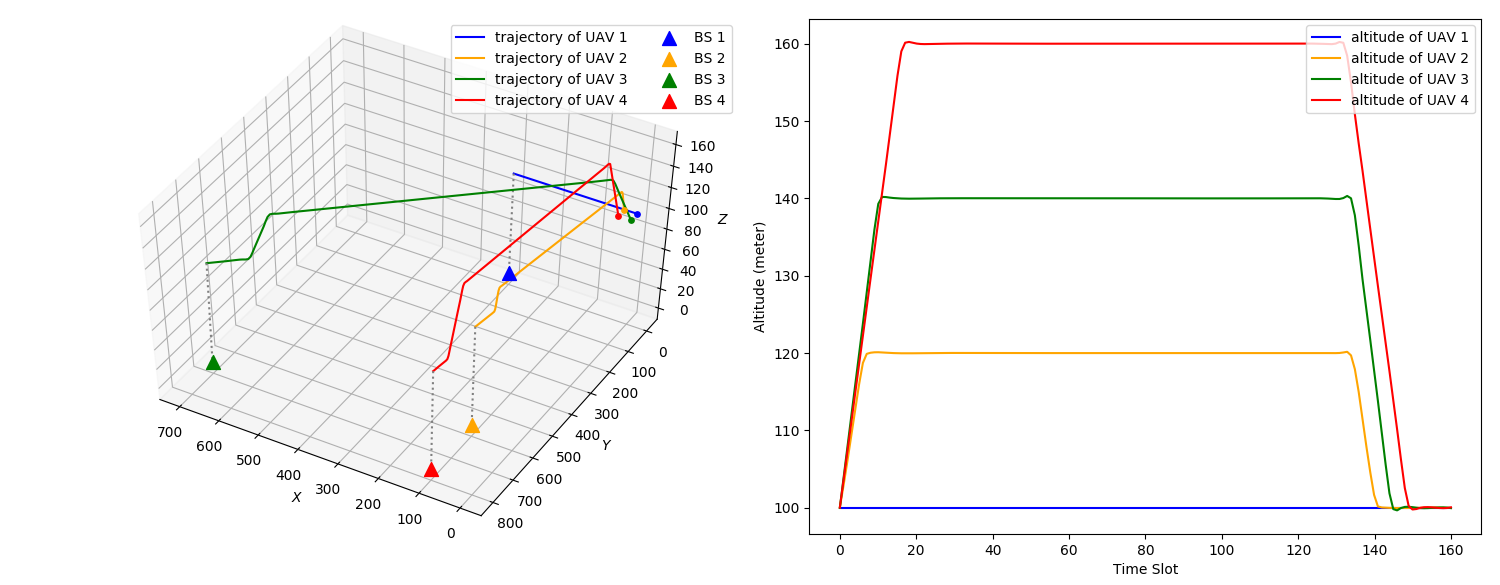
\includegraphics[width=\linewidth]{init_trajectory.png}
	\caption{Initial trajectory}
\end{figure}
Figure 1 illustrates our initial trajectory with altitude that follows the setup strategy above, and unless otherwise stated, the initial locations for UAVs in our simulation are (0, 0, 100), (30, 0, 100), (0, 30, 100), and (30, 30, 100), along with the initial locations for base stations are (300, 0, 0), (100, 600, 0), (700, 700, 0) and (100, 800, 0). Initially, all the UAVs use the maximum transmission power to communicate with the serving base stations. \\ \par 

\textit{C. Optimization Result} \par 
Initially, the algorithm requires a set of hovering positions to start the optimization, and by solving (10) one can see that the optimized hovering positions of UAVs are all near to their serving base stations, and also the hovering altitude are all close to the minimum height. \par  

Then we put the initial trajectory and the pre-defined parameters into our simulation programs for iterations, and obtain an optimized trajectory shown in figure 2, as well as an optimized power control for each UAV. Intuitively, one can see from the optimization result is that the maximum altitudes of UAVs are lower compared with the initial trajectory. 
\begin{figure}[H]
	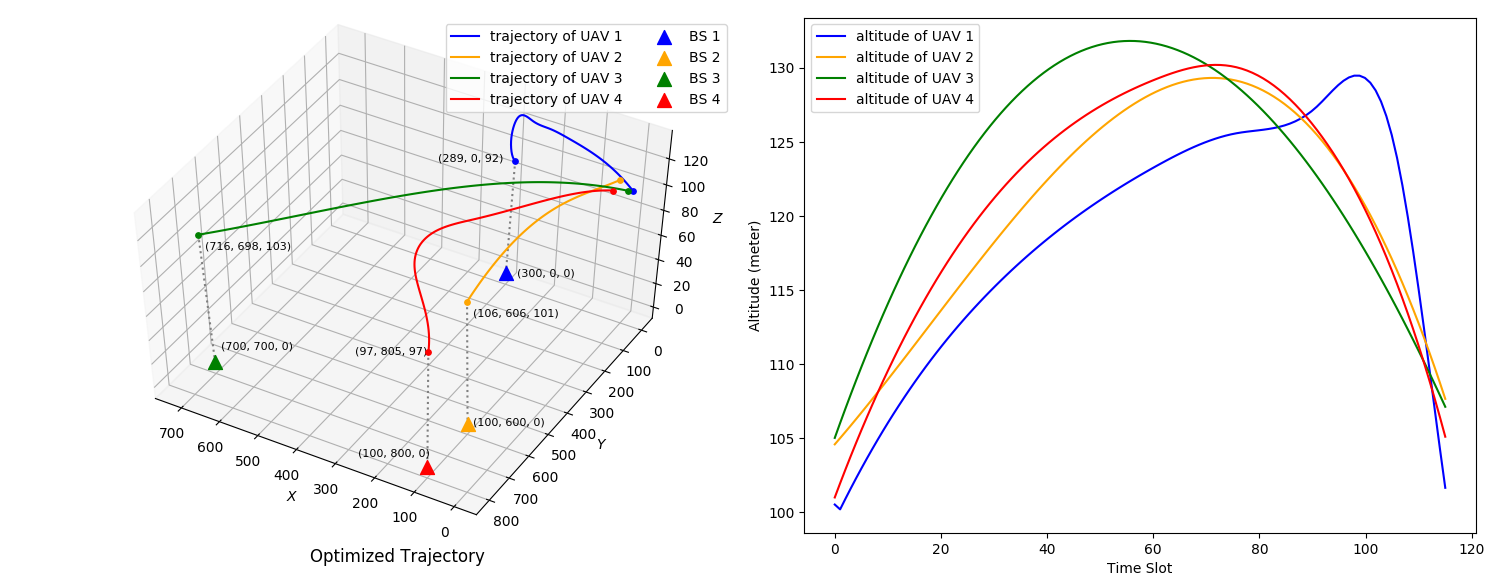
\includegraphics[width=\linewidth]{opt_trajectory.png}
	\caption{Optimized trajectory}
\end{figure}
Specifically, as observed from the figure, UAV 1 is initially close to its destination and it reaches its destination with a short traveling time compared with the other UAVs. As it reaches the close x-y coordinate of its serving base station, UAV 1 does not immediately descend to its optimal height but keeps its altitude and waits for the UAVs which takes more traveling time to reach their serving base stations. Then these four UAVs start descending to their optimal hovering points at almost simultaneously so as to avoid the addictive interference from the UAV which descends earlier than the others. From the optimized trajectory one can see that the optimization does not only avoid the collision between UAVs, but also schedules a coordination among the UAVs. \par 
By formula (6), the corresponding aggregate achievable transmission rates can be calculated. The plot of achievable transmission rates at different time slots is shown as figure 3. Initially, the maximum aggregate achievable transmission of four UAVs are around 3.5 bit per second. After the optimization, one can see that the maximum aggregate achievable transmission rate accedes 11 bit per second, which is 3 times larger compared with the initial achievable rate. Also, UAVs take less time to attain the steady state at the maximum transmission rate compared with the initial setup. 
\begin{figure}[H]
	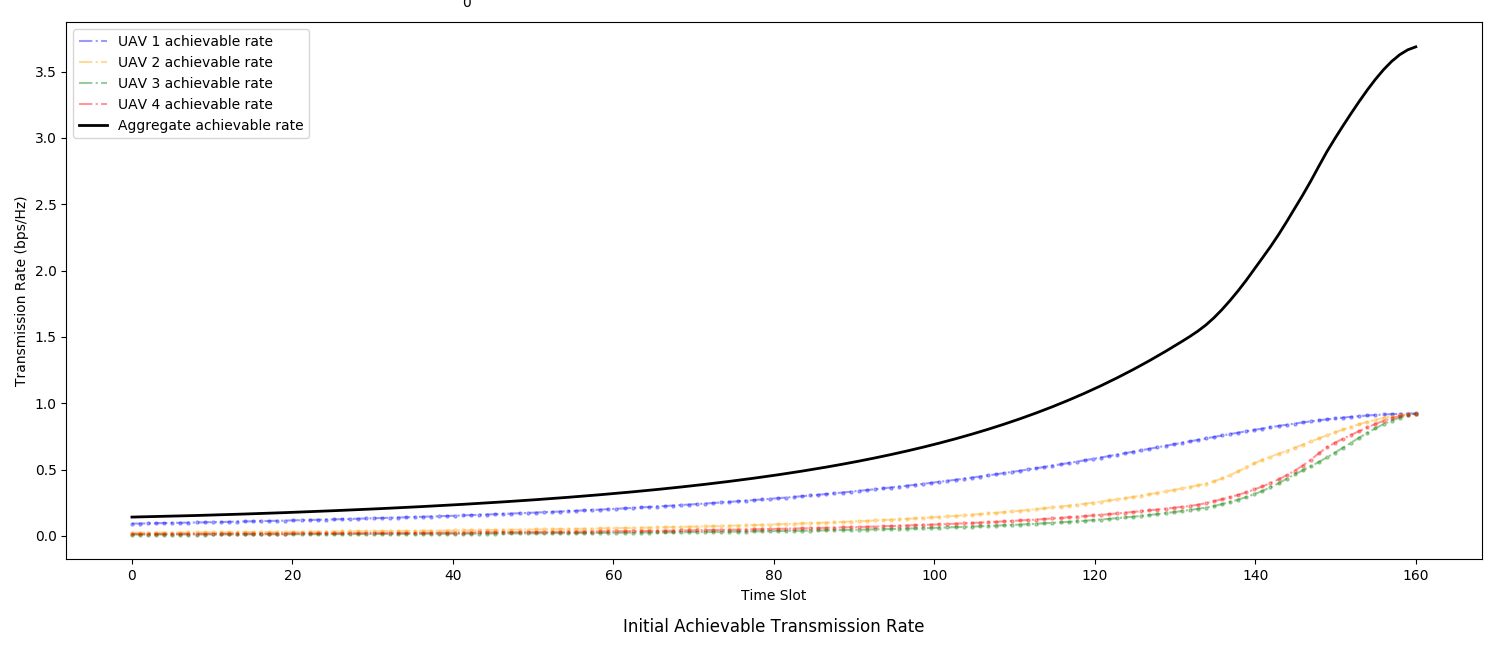
\includegraphics[width=\linewidth]{init_rate.png}
	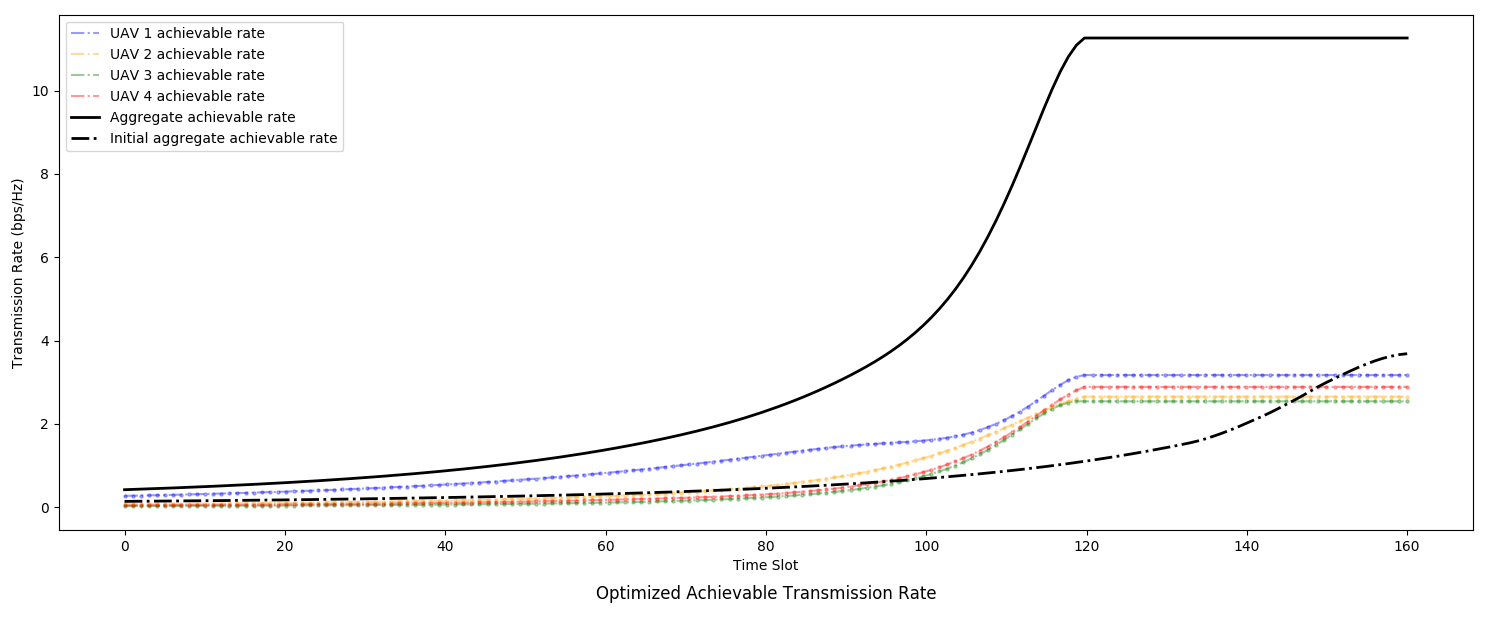
\includegraphics[width=\linewidth]{opt_rate.png}
	\caption{Achievable transmission rate}
\end{figure}


\section{Conclusion}\label{VI}
In this paper, we have studied the joint trajectory and power control design for UAVs. In general, TPC problem is a NP-hard problem, and a heuristic and sub-optimal algorithms have been purposed in this paper to jointly optimize the initial trajectory and power control. We utilize the Taylor expansion to find the local optimal for non-convex functions involved in the TPC problem and also give several solid algorithms to obtain the result for the related optimization problems. From the simulation we conclude that our algorithm is feasible in handling the TPC problem. The aggregate achievable transmission rate raised and the UAVs approached the destinations by a more preferable route after the optimization. \par 
The current work can be extended to several different directions. First, in this paper we assume that the Doppler effect can be ignored, while it might be a significant factor in evaluating the achievable transmission rate if UAVs are allowed to fly at a fast speed, thus it is necessary to improve our algorithm in order to guarantee the robustness of our algorithm in more sophisticated scenarios. Second, in the simulation we found that the centralized algorithm requires a huge amount of time to compute the result, and if the scale of the problem gets larger, the total computation time could be increase fast. One possible solution is to apply ADMM algorithm to modify the SCA-based algorithm to reduce the computation overhead by parallel computing. 


\section{Acknowledgment}
This report are mainly based on paper written by Chao Shen, Tsung-Hui Chang, Jie Gong, Yong Zeng, and Rui Zhang \cite{IEEEexample:shen2018multi}. We correct the errors in orginial paper, modify the two lemmas and provide rigorous proof for them. The method to find minimum number of time slots $M$ and initial trajectory (including Algorithm \ref{alg:2} for checking feasibility) is proposed by us.




\bibliographystyle{IEEEtran}
\bibliography{IEEEabrv,IEEEexample}


\end{document}
